\documentclass{beamer}

\usepackage{tikz}
\usetikzlibrary{calc,backgrounds}
\usepackage{amsmath}
\usepackage{amssymb}
\usepackage{float}
\usepackage{graphicx}
\usepackage{svg}
\usepackage{pgfplots}
\usepackage{xcolor}
\usepackage{subcaption}

\setcounter{MaxMatrixCols}{20} % Increase max allowed columns

\usetikzlibrary{fadings}
\tikzfading
  [name=fadeLR,
   left color=transparent!100,  % fully transparent at the left
   right color=transparent!0]   % fully opaque at the right
\tikzfading
   [name=fadeRL,
    right color=transparent!100,  % fully transparent at the left
    left color=transparent!0]   % fully opaque at the right

\definecolor{pale_yellow}{HTML}{ffef96}

\definecolor{col1}{HTML}{7570B3}
\definecolor{col2}{HTML}{D95F02}
\definecolor{col3}{HTML}{1B9E77}
\definecolor{col4}{HTML}{E7298A}
\definecolor{col5}{HTML}{66A61E}
\definecolor{col6}{HTML}{E6AB02}

\definecolor{col1_light}{HTML}{8f8ac0}
\definecolor{col2_light}{HTML}{d88a5f}
\definecolor{col3_light}{HTML}{6fb89f}
\definecolor{col4_light}{HTML}{e08fb5}
\definecolor{col5_light}{HTML}{8fb87f}
\definecolor{col6_light}{HTML}{e0c15a}

\setbeamertemplate{footline}[frame number]

\title{Structuring Echo State Networks using Ordinal Partitions}% TODO title
\author{Hector Morlet\\22247737\\Supervised by Eugene Tan, Michael Small}
\date{March 14, 2025}

\begin{document}


\frame{\titlepage} % Title slide

% Introduction
\begin{frame}
    \frametitle{Introduction}
    \begin{itemize}
        \item Echo State Networks
        \item Ordinal Partitions
        \item 2 Main Research Proposals
    \end{itemize}
\end{frame}

% Echo state networks
\begin{frame}
    \frametitle{Echo State Networks}
    \begin{itemize}
        \item First introduced by Jaeger (2001). %TODO reference
        \item Type of recurrent neural network.
        \item Commonly studied form of reservoir computing.
        \item A form of supervised learning.
        \item Most weights are fixed and only some are fitted.
        \item Is computationally efficient compared to other neural networks.
    \end{itemize}
\end{frame}

% Echo state Networks
\begin{frame}
    \frametitle{Echo State Networks}
    State update equation:
    \[
        \mathbf{s}(t + 1) = f_{act}(\mathbf{W}_{in}x(t) + \mathbf{W}_{rec}\mathbf{s}(t) + \mathbf{W}_{bias})
    \]
    \begin{itemize}
        % \begin{itemize}
        %     \item Given a sufficiently long input sequence, the current state of the reservoir is determined uniquely by the intervening input and is independent of its initial state.
        % \end{itemize} % TODO reference here
        \item $\mathbf{W}_{in}$, $\mathbf{W}_{rec}$, $\mathbf{W}_{bias}$ and $\mathbf{s}(t)$ are randomly generated according to hyper-parameters.
        % \item $\mathbf{W}_{rec}$ is a randomly generated network weight matrix (e.g. Erdos-Renyi).
        \item Echo state property
        \item $\mathbf{W}_{in}$, $\mathbf{W}_{rec}$ and $\mathbf{W}_{bias}$ are fixed.
        \item Only the readout vector weights is fitted. % TODO reference A practical guide to applying echo state networks
    \end{itemize}
\end{frame}

% Echo state networks
\begin{frame}
    \frametitle{Echo State Networks}

    Output equation:
    \[
        y(t) = \mathbf{C}_{out}\mathbf{s}(t)
    \]
    \[
        \mathbf{Y} = \mathbf{C}_{out}\mathbf{S}
    \]

    Output regression with regularisation: % TODO reference [4] in Lucas'
    \[
        \mathbf{C}_{out} = (\mathbf{S}^T \mathbf{S} + \beta \mathbf{I}) \ \mathbf{S}^T \mathbf{Y}
    \]

    \begin{figure}
        
    %     \centering
        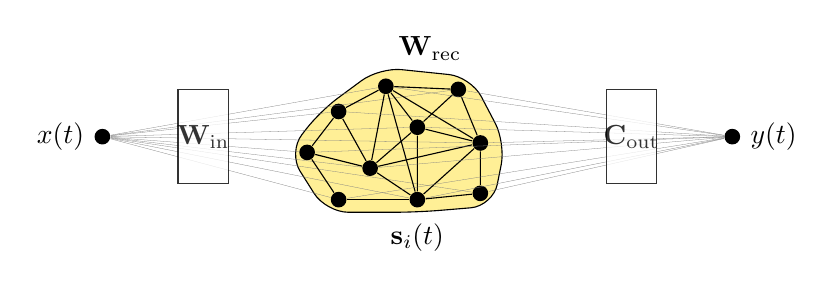
\begin{tikzpicture}[scale=0.8]
            \node[fill=black,circle,inner sep=2pt,label=left:$x(t)$] (input) at (0,0) {};
            \node[fill=black,circle,inner sep=2pt,label=right:$y(t)$] (output) at (10,0) {};
            
            
            \coordinate (res_anchor) at (2,3);
            \node[fill=black,circle,inner sep=2pt] (res1) at ({5-0.5},{0.8}) {};
            \node[fill=black,circle,inner sep=2pt] (res2) at ({5},{-1}) {};
            \node[fill=black,circle,inner sep=2pt] (res3) at ({5},{0.15}) {};
            \node[fill=black,circle,inner sep=2pt] (res4) at ({5+1},{-0.1}) {};
            \node[fill=black,circle,inner sep=2pt] (res5) at ({5-0.75},{-0.5}) {};
            \node[fill=black,circle,inner sep=2pt] (res6) at ({5-1.25},{0.4}) {};
            \node[fill=black,circle,inner sep=2pt] (res7) at ({5+0.65},{0.75}) {};
            \node[fill=black,circle,inner sep=2pt] (res8) at ({5+1},{-0.9}) {};
            \node[fill=black,circle,inner sep=2pt] (res9) at ({5-1.25},{-1}) {};
            \node[fill=black,circle,inner sep=2pt] (res10) at ({5-1.75},{-0.25}) {};
        
            \foreach \i in {1,...,10}
                \draw[gray,line width=0.1] (input) -- (res\i);
            
            \foreach \i in {1,...,5}
                \foreach \j in {1,...,5} {
                    \ifnum\i<\j
                        \draw (res\i) -- (res\j);
                    \fi
                }
            
            \draw (res6) -- (res5);
            \draw (res6) -- (res1);
            \draw (res6) -- (res10);
            \draw (res10) -- (res5);
            \draw (res9) -- (res10);
            \draw (res9) -- (res2);
            \draw (res7) -- (res1);
            \draw (res7) -- (res3);
            \draw (res7) -- (res4);
            \draw (res8) -- (res4);
            \draw (res8) -- (res2);
            
            \foreach \i in {1,...,10}
                \draw[gray,line width=0.1] (res\i) -- (output);
            
            \begin{scope}[on background layer]
            \draw[draw=black,fill=pale_yellow,rounded corners=8pt]  ($(res1)+(-0.1,0.3)$) -- ($(res7)+(+0.2,+0.2)$) -- ($(res4)+(0.4,0)$) -- ($(res8)+(0.2,-0.2)$) -- ($(res2)+(0,-0.2)$) -- ($(res9)+(-0.2,-0.2)$) -- ($(res10)+(-0.3,0)$) -- ($(res6)+(-0.3,0)$) -- cycle;
            \end{scope}
            \node at (5.2, 1.4) {$\mathbf{W}_{\text{rec}}$};
            \node at (5, -1.6) {$\mathbf{s}_i(t)$};
            
            \draw[fill=white,opacity=0.8] (1.2,-0.75) rectangle (2.0,0.75) node[midway] {$\mathbf{W}_{\text{in}}$};
            \draw[fill=white,opacity=0.8] (8, -0.75) rectangle (8.8,0.75) node[midway] {$\mathbf{C}_{\text{out}}$};
        \end{tikzpicture}
        \caption{A diagram of an Echo State Network.}
        \label{fig:ESN}
    \end{figure}
\end{frame}

% Ordinal partitions
\begin{frame}
    \frametitle{Ordinal Partitions}

    \begin{itemize}
        \item Bandt and Pompe (2002).
        \item Each data point in a timeseries is partitioned by the ordering of its preceding points.
        \item Each partition has a unique `ordinal symbol' (e.g. numbers from 1 to 6).
        \item The probability of the timeseries transitioning from one partition to another can be calculated, giving the `ordinal transition probabilities'.
    \end{itemize}
\end{frame}

% Ordinal partitions
\begin{frame}
    \frametitle{Ordinal Partitions}

    % \begin{itemize}
    %     \item Each point in a timeseries is categorised by the ranking of its preceding points.
    % \end{itemize}
    
    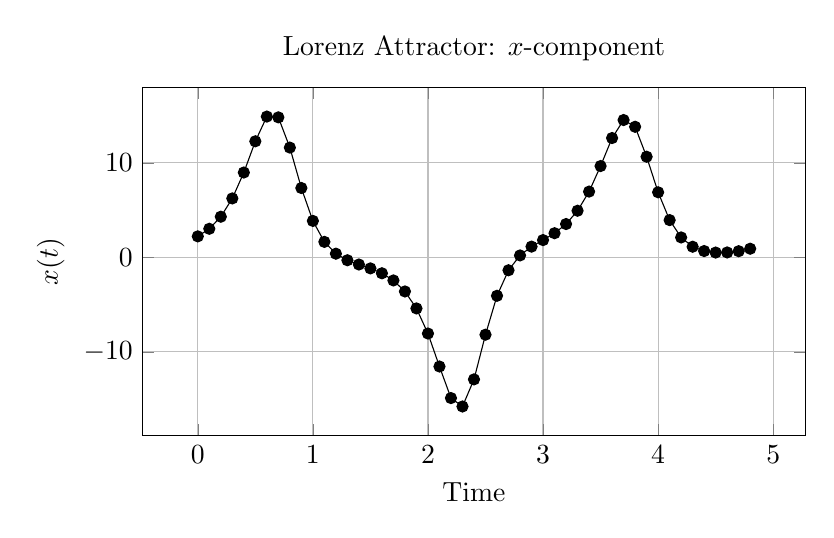
\begin{tikzpicture}
        \begin{axis}[
          xlabel={Time},
          ylabel={$x(t)$},
          title={Lorenz Attractor: $x$-component},
          width=10cm, height=6cm,
          grid=major
        ]
          % Data generated by solving dx/dt = sigma(y - x), etc. in Python
          \addplot[black, mark=*, mark options={black}] coordinates {
            (0.0, 2.2165566502619796)
            (0.1, 3.0181360987381685)
            (0.2, 4.2948078524935065)
            (0.3, 6.231121537780632)
            (0.4, 8.970926893912857)
            (0.5, 12.272230400810887)
            (0.6, 14.887997312478161)
            (0.7, 14.803117347063516)
            (0.8, 11.606868473299526)
            (0.9, 7.330990437181266)
            (1.0, 3.85191889651296)
            (1.1, 1.6347534154776406)
            (1.2, 0.3853895148599277)
            (1.3, -0.30838099414996695)
            (1.4, -0.7586726217449103)
            (1.5, -1.1695821908357407)
            (1.6, -1.6858338981790886)
            (1.7, -2.443141458426554)
            (1.8, -3.6086854451117074)
            (1.9, -5.40339197322587)
            (2.0, -8.058505977971057)
            (2.1, -11.547145254692042)
            (2.2, -14.884182443761347)
            (2.3, -15.775516623377253)
            (2.4, -12.908181797239536)
            (2.5, -8.181376578133673)
            (2.6, -4.06724026097539)
            (2.7, -1.3665393788429014)
            (2.8, 0.20110496364168012)
            (2.9, 1.1324784341364973)
            (3.0, 1.8245674314417792)
            (3.1, 2.5516132966355554)
            (3.2, 3.5214281335608555)
            (3.3, 4.926987945369609)
            (3.4, 6.951562500713474)
            (3.5, 9.654345729238477)
            (3.6, 12.617195234374243)
            (3.7, 14.521825487882024)
            (3.8, 13.806356286601272)
            (3.9, 10.64113968132102)
            (4.0, 6.880279139891668)
            (4.1, 3.9367704788159394)
            (4.2, 2.1029851064946445)
            (4.3, 1.121305395878461)
            (4.4, 0.665491176850325)
            (4.5, 0.5051437108082056)
            (4.6, 0.5156168027361644)
            (4.7, 0.6490783162490397)
            (4.8, 0.9105168761220792)
          };
        \end{axis}
      \end{tikzpicture}    
\end{frame}

% Ordinal partitions
\begin{frame}
    \frametitle{Ordinal Partitions}

    \begin{center}
        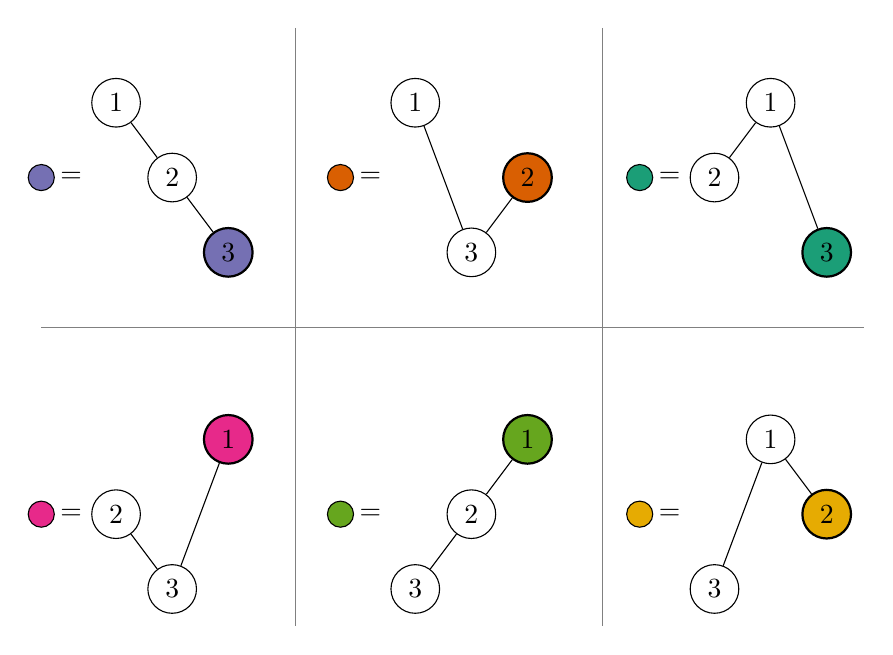
\begin{tikzpicture}[scale=0.95]
            % partition 1

            \node[circle, draw, fill=col1] (topleft) at (-5.0, 3) {};

            % Draw the equality sign
            \node at (-4.6, 3) {$=$};
            
            % Draw the nodes in the lower part
            \node[circle, draw] (1_2) at (-4.0, 4) {1};
            \node[circle, draw] (1_1) at (-3.25, 3) {2};
            \node[circle, draw, thick, fill=col1] (1_3) at (-2.5, 2) {3};
            
            % Draw edges
            \draw (1_1) -- (1_2);
            \draw (1_1) -- (1_3);

            % Draw dividing line
            \draw[gray, very thin] (-1.6, 5) -- (-1.6, -3);

            % partition 2

            \node[circle, draw, fill=col2] (topcentre) at (-1, 3) {};

            % Draw the equality sign
            \node at (-0.6, 3) {$=$};
            
            % Draw the nodes in the lower part
            \node[circle, draw] (2_2) at (0, 4) {1};
            \node[circle, draw] (2_1) at (0.75, 2) {3};
            \node[circle, draw, thick, fill=col2] (2_3) at (1.5, 3) {2};
            
            % Draw edges
            \draw (2_1) -- (2_2);
            \draw (2_1) -- (2_3);

            % Draw dividing line
            \draw[gray, very thin] (2.5, 5) -- (2.5, -3);

            % partition 3

            \node[circle, draw, fill=col3] (topleft) at (3.0, 3) {};

            % Draw the equality sign
            \node at (3.4, 3) {$=$};
            
            % Draw the nodes in the lower part
            \node[circle, draw] (3_2) at (4.0, 3) {2};
            \node[circle, draw] (3_1) at (4.75, 4) {1};
            \node[circle, draw, thick, fill=col3] (3_3) at (5.5, 2) {3};
            
            % Draw edges
            \draw (3_1) -- (3_2);
            \draw (3_1) -- (3_3);

            % Draw dividing line
            \draw[gray, very thin] (-5, 1) -- (6, 1);

            % partition 4

            \node[circle, draw, fill=col4] (bottomleft) at (-5.0, -1.5) {};

            % Draw the equality sign
            \node at (-4.6, -1.5) {$=$};
            
            % Draw the nodes in the lower part
            \node[circle, draw] (4_2) at (-4.0, -1.5) {2};
            \node[circle, draw] (4_1) at (-3.25, -2.5) {3};
            \node[circle, draw, thick, fill=col4] (4_3) at (-2.5, -0.5) {1};
            
            % Draw edges
            \draw (4_1) -- (4_2);
            \draw (4_1) -- (4_3);

            % Draw dividing line
            % \draw[gray, very thin] (-2.25, -3) -- (-2.25, -5);

            % partition 5

            \node[circle, draw, fill=col5] (bottomcentre) at (-1, -1.5) {};

            % Draw the equality sign
            \node at (-0.6, -1.5) {$=$};
            
            % Draw the nodes in the lower part
            \node[circle, draw] (5_2) at (0, -2.5) {3};
            \node[circle, draw] (5_1) at (0.75, -1.5) {2};
            \node[circle, draw, thick, fill=col5] (5_3) at (1.5, -0.5) {1};
            
            % Draw edges
            \draw (5_1) -- (5_2);
            \draw (5_1) -- (5_3);

            % partition 6

            \node[circle, draw, fill=col6] (bottomright) at (3.0, -1.5) {};

            % Draw the equality sign
            \node at (3.4, -1.5) {$=$};
            
            % Draw the nodes in the lower part
            \node[circle, draw] (6_2) at (4.0, -2.5) {3};
            \node[circle, draw] (6_1) at (4.75, -0.5) {1};
            \node[circle, draw, thick, fill=col6] (6_3) at (5.5, -1.5) {2};
            
            % Draw edges
            \draw (6_1) -- (6_2);
            \draw (6_1) -- (6_3);
        \end{tikzpicture}
    \end{center}
\end{frame}

% Ordinal partitions
\begin{frame}
    \frametitle{Ordinal Partitions}
    
      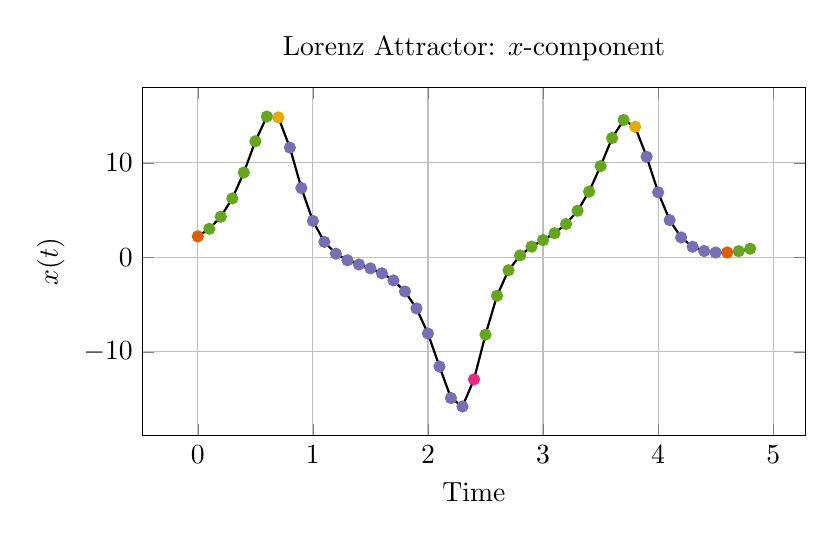
\begin{tikzpicture}
        \begin{axis}[
            xlabel={Time},
            ylabel={$x(t)$},
            title={Lorenz Attractor: $x$-component},
            width=10cm, height=6cm,
            grid=major
        ]


        \addplot [
            thick, % or any style you like
        ] coordinates {
            (0.0, 2.2165566502619796)
            (0.1, 3.0181360987381685)
            (0.2, 4.2948078524935065)
            (0.3, 6.231121537780632)
            (0.4, 8.970926893912857)
            (0.5, 12.272230400810887)
            (0.6, 14.887997312478161)
            (0.7, 14.803117347063516)
            (0.8, 11.606868473299526)
            (0.9, 7.330990437181266)
            (1.0, 3.85191889651296)
            (1.1, 1.6347534154776406)
            (1.2, 0.3853895148599277)
            (1.3, -0.30838099414996695)
            (1.4, -0.7586726217449103)
            (1.5, -1.1695821908357407)
            (1.6, -1.6858338981790886)
            (1.7, -2.443141458426554)
            (1.8, -3.6086854451117074)
            (1.9, -5.40339197322587)
            (2.0, -8.058505977971057)
            (2.1, -11.547145254692042)
            (2.2, -14.884182443761347)
            (2.3, -15.775516623377253)
            (2.4, -12.908181797239536)
            (2.5, -8.181376578133673)
            (2.6, -4.06724026097539)
            (2.7, -1.3665393788429014)
            (2.8, 0.20110496364168012)
            (2.9, 1.1324784341364973)
            (3.0, 1.8245674314417792)
            (3.1, 2.5516132966355554)
            (3.2, 3.5214281335608555)
            (3.3, 4.926987945369609)
            (3.4, 6.951562500713474)
            (3.5, 9.654345729238477)
            (3.6, 12.617195234374243)
            (3.7, 14.521825487882024)
            (3.8, 13.806356286601272)
            (3.9, 10.64113968132102)
            (4.0, 6.880279139891668)
            (4.1, 3.9367704788159394)
            (4.2, 2.1029851064946445)
            (4.3, 1.121305395878461)
            (4.4, 0.665491176850325)
            (4.5, 0.5051437108082056)
            (4.6, 0.5156168027361644)
            (4.7, 0.6490783162490397)
            (4.8, 0.9105168761220792)
        };
        
        
        % Define how each "class" (symbolic label) is colored and drawn:
        \addplot[
            scatter,
            only marks,
            scatter src=explicit symbolic,
            scatter/classes={
                1={mark=*,draw=col1,fill=col1},
                2={mark=*,draw=col2,fill=col2},
                3={mark=*,draw=col3,fill=col3},
                4={mark=*,draw=col4,fill=col4},
                5={mark=*,draw=col5,fill=col5},
                6={mark=*,draw=col6,fill=col6}
            }
        ] 
        coordinates {
            (0.0, 2.2165566502619796)[2]
            (0.1, 3.0181360987381685)[5]
            (0.2, 4.2948078524935065)[5]
            (0.3, 6.231121537780632)[5]
            (0.4, 8.970926893912857)[5]
            (0.5, 12.272230400810887)[5]
            (0.6, 14.887997312478161)[5]
            (0.7, 14.803117347063516)[6]
            (0.8, 11.606868473299526)[1]
            (0.9, 7.330990437181266)[1]
            (1.0, 3.85191889651296)[1]
            (1.1, 1.6347534154776406)[1]
            (1.2, 0.3853895148599277)[1]
            (1.3, -0.30838099414996695)[1]
            (1.4, -0.7586726217449103)[1]
            (1.5, -1.1695821908357407)[1]
            (1.6, -1.6858338981790886)[1]
            (1.7, -2.443141458426554)[1]
            (1.8, -3.6086854451117074)[1]
            (1.9, -5.40339197322587)[1]
            (2.0, -8.058505977971057)[1]
            (2.1, -11.547145254692042)[1]
            (2.2, -14.884182443761347)[1]
            (2.3, -15.775516623377253)[1]
            (2.4, -12.908181797239536)[4]
            (2.5, -8.181376578133673)[5]
            (2.6, -4.06724026097539)[5]
            (2.7, -1.3665393788429014)[5]
            (2.8, 0.20110496364168012)[5]
            (2.9, 1.1324784341364973)[5]
            (3.0, 1.8245674314417792)[5]
            (3.1, 2.5516132966355554)[5]
            (3.2, 3.5214281335608555)[5]
            (3.3, 4.926987945369609)[5]
            (3.4, 6.951562500713474)[5]
            (3.5, 9.654345729238477)[5]
            (3.6, 12.617195234374243)[5]
            (3.7, 14.521825487882024)[5]
            (3.8, 13.806356286601272)[6]
            (3.9, 10.64113968132102)[1]
            (4.0, 6.880279139891668)[1]
            (4.1, 3.9367704788159394)[1]
            (4.2, 2.1029851064946445)[1]
            (4.3, 1.121305395878461)[1]
            (4.4, 0.665491176850325)[1]
            (4.5, 0.5051437108082056)[1]
            (4.6, 0.5156168027361644)[2]
            (4.7, 0.6490783162490397)[5]
            (4.8, 0.9105168761220792)[5]
        };
        
        \end{axis}
        \end{tikzpicture}
\end{frame}

% Ordinal partitions
\begin{frame}
    \frametitle{Ordinal Partitions}
    \begin{table}[]
        \centering
        \begin{tabular}{c|cccccc}
            & \tikz\draw[fill=col1,draw=col1] (0,0) circle (0.9ex); 
            & \tikz\draw[fill=col2,draw=col2] (0,0) circle (0.9ex); 
            & \tikz\draw[fill=col3,draw=col3] (0,0) circle (0.9ex); 
            & \tikz\draw[fill=col4,draw=col4] (0,0) circle (0.9ex); 
            & \tikz\draw[fill=col5,draw=col5] (0,0) circle (0.9ex); 
            & \tikz\draw[fill=col6,draw=col6] (0,0) circle (0.9ex); \\ \hline
            \tikz\draw[fill=col1,draw=col1] (0,0) circle (0.9ex); & 0.7 & 0.1 & 0.1 & 0.05 & 0.05 & 0.0 \\
            \tikz\draw[fill=col2,draw=col2] (0,0) circle (0.9ex); & 0.0 & 0.0 & 0.0 & 0.0 & 0.9 & 0.1 \\
            \tikz\draw[fill=col3,draw=col3] (0,0) circle (0.9ex); & 0.7 & 0.1 & 0.1 & 0.05 & 0.05 & 0.0 \\
            \tikz\draw[fill=col4,draw=col4] (0,0) circle (0.9ex); & 0.0 & 0.0 & 0.0 & 0.0 & 0.9 & 0.1 \\
            \tikz\draw[fill=col5,draw=col5] (0,0) circle (0.9ex); & 0.0 & 0.0 & 0.0 & 0.0 & 0.9 & 0.1 \\
            \tikz\draw[fill=col6,draw=col6] (0,0) circle (0.9ex); & 0.7 & 0.05 & 0.05 & 0.05 & 0.05 & 0.1 \\
        \end{tabular}
        \caption{Transition probabilities between ordinal partitions.}
        \label{tab:transition_probabilities}
    \end{table}
\end{frame}

% Research Questions
\begin{frame}
    \frametitle{Research Questions}
    \begin{itemize}
        % \item few improvements can be made on ESN's... % TODO find reference
        % \item Prior studies suggest that `stacking reservoirs' can broaden the range of dynamics an ESN an capture. % TODO cite https://arxiv.org/abs/2105.06923#:~:text=determines%20the%20performance%20of%20the,later%20stage%20of%20the%20deep
        \item Can ordinal partitions be used to improve forecasting accuracy?
        \item `Feature selection'
        % \item Interpretability
    \end{itemize}
\end{frame}

% Input data
\begin{frame}
    \frametitle{Input data: Lorenz}

    \[
    \begin{aligned}
        \frac{dx}{dt} &= \sigma (y - x) \\
        \frac{dy}{dt} &= x (\rho - z) - y \\
        \frac{dz}{dt} &= xy - \beta z
    \end{aligned}
    \]

    \begin{figure}
        \centering
        \begin{minipage}{0.5\textwidth}
            \centering
            \includegraphics[width=\textwidth]{Lorenz_component.png}
        \end{minipage}%
        \begin{minipage}{0.5\textwidth}
            \centering
            \includegraphics[width=\textwidth]{Lorenz_3d.png}
        \end{minipage}
        % \caption{Visualization of the Lorenz component and 3D visualization of the Lorenz attractor.}
        \label{fig:lorenz_combined}
    \end{figure}
\end{frame}

% % Research proposals
% \begin{frame}
%     \frametitle{Research Proposals}

%     \begin{itemize}
%         \item \textbf{Approach 1}: switch the readout ($C_{out}$) vector based on the ordinal partition.
%         \item \textbf{Approach 2}: restructure the reservoir into subreservoirs for each partition.
%         \begin{itemize}
%             \item Feed the input based on the ordinal partition.
%             \item Weight the connections between subreservoirs according to the transition probabilities of the ordinal network.
%         \end{itemize}
%         \item \textbf{Approach 2.2}: Stochastic partitioned ESN.
%         \begin{itemize}
%             \item Each time step, for each subreservoir, choose one other subreservoir to connect to based on the transition probabilities of the ordinal network.
%             \item Only connect to that subreservoir and do not connect to any of the other subreservoirs.
%         \end{itemize}
%     \end{itemize}
% \end{frame}

% Research proposal: Approach 1
\begin{frame}
    \frametitle{Research Proposal: Approach 1}

    % C_{out} = C_{part}[:, P(t)]
    Switch the readout ($C_{out}$) vector based on the ordinal partition.

    \begin{figure}
        
    %     \centering
        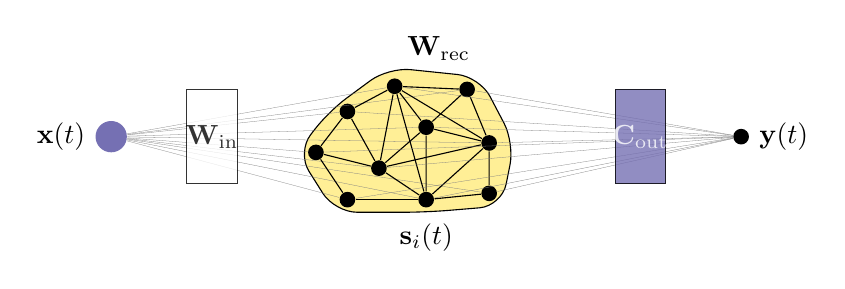
\begin{tikzpicture}[scale=0.8]
            \node[fill=col1,circle,inner sep=4pt,label=left:$\mathbf{x}(t)$] (input) at (0,0) {};
            \node[fill=black,circle,inner sep=2pt,label=right:$\mathbf{y}(t)$] (output) at (10,0) {};
            
            
            \coordinate (res_anchor) at (2,3);
            \node[fill=black,circle,inner sep=2pt] (res1) at ({5-0.5},{0.8}) {};
            \node[fill=black,circle,inner sep=2pt] (res2) at ({5},{-1}) {};
            \node[fill=black,circle,inner sep=2pt] (res3) at ({5},{0.15}) {};
            \node[fill=black,circle,inner sep=2pt] (res4) at ({5+1},{-0.1}) {};
            \node[fill=black,circle,inner sep=2pt] (res5) at ({5-0.75},{-0.5}) {};
            \node[fill=black,circle,inner sep=2pt] (res6) at ({5-1.25},{0.4}) {};
            \node[fill=black,circle,inner sep=2pt] (res7) at ({5+0.65},{0.75}) {};
            \node[fill=black,circle,inner sep=2pt] (res8) at ({5+1},{-0.9}) {};
            \node[fill=black,circle,inner sep=2pt] (res9) at ({5-1.25},{-1}) {};
            \node[fill=black,circle,inner sep=2pt] (res10) at ({5-1.75},{-0.25}) {};
        
            \foreach \i in {1,...,10}
                \draw[gray,line width=0.1] (input) -- (res\i);
            
            \foreach \i in {1,...,5}
                \foreach \j in {1,...,5} {
                    \ifnum\i<\j
                        \draw (res\i) -- (res\j);
                    \fi
                }
            
            \draw (res6) -- (res5);
            \draw (res6) -- (res1);
            \draw (res6) -- (res10);
            \draw (res10) -- (res5);
            \draw (res9) -- (res10);
            \draw (res9) -- (res2);
            \draw (res7) -- (res1);
            \draw (res7) -- (res3);
            \draw (res7) -- (res4);
            \draw (res8) -- (res4);
            \draw (res8) -- (res2);
            
            \foreach \i in {1,...,10}
                \draw[gray,line width=0.1] (res\i) -- (output);
            
            \begin{scope}[on background layer]
            \draw[draw=black,fill=pale_yellow,rounded corners=8pt]  ($(res1)+(-0.1,0.3)$) -- ($(res7)+(+0.2,+0.2)$) -- ($(res4)+(0.4,0)$) -- ($(res8)+(0.2,-0.2)$) -- ($(res2)+(0,-0.2)$) -- ($(res9)+(-0.2,-0.2)$) -- ($(res10)+(-0.3,0)$) -- ($(res6)+(-0.3,0)$) -- cycle;
            \end{scope}
            \node at (5.2, 1.4) {$\mathbf{W}_{\text{rec}}$};
            \node at (5, -1.6) {$\mathbf{s}_i(t)$};
            
            \draw[fill=white,opacity=0.8] (1.2,-0.75) rectangle (2.0,0.75) node[midway] {$\mathbf{W}_{\text{in}}$};
            \draw[fill=col1,opacity=0.8] (8, -0.75) rectangle (8.8,0.75) node[midway, text=white] {$\mathbf{C}_{\text{out}}$};
        \end{tikzpicture}
        \caption{Echo State Network with readout switching.}
        \label{fig:ESN}
    \end{figure}
\end{frame}

% Research proposal: Approach 1
\begin{frame}
    \frametitle{Research Proposal: Approach 1}

    Switch the readout ($C_{out}$) vector based on the ordinal partition.

    \begin{figure}
        
    %     \centering
        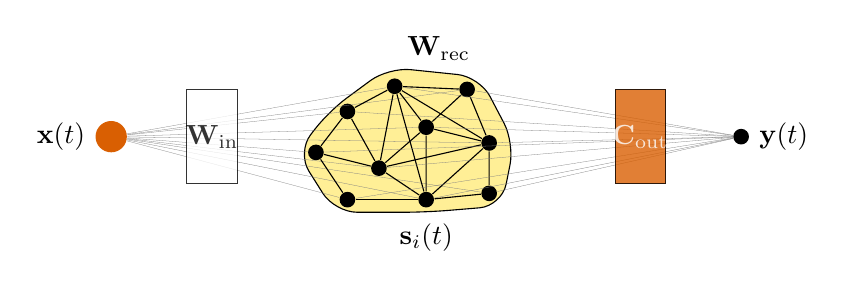
\begin{tikzpicture}[scale=0.8]
            \node[fill=col2,circle,inner sep=4pt,label=left:$\mathbf{x}(t)$] (input) at (0,0) {};
            \node[fill=black,circle,inner sep=2pt,label=right:$\mathbf{y}(t)$] (output) at (10,0) {};
            
            
            \coordinate (res_anchor) at (2,3);
            \node[fill=black,circle,inner sep=2pt] (res1) at ({5-0.5},{0.8}) {};
            \node[fill=black,circle,inner sep=2pt] (res2) at ({5},{-1}) {};
            \node[fill=black,circle,inner sep=2pt] (res3) at ({5},{0.15}) {};
            \node[fill=black,circle,inner sep=2pt] (res4) at ({5+1},{-0.1}) {};
            \node[fill=black,circle,inner sep=2pt] (res5) at ({5-0.75},{-0.5}) {};
            \node[fill=black,circle,inner sep=2pt] (res6) at ({5-1.25},{0.4}) {};
            \node[fill=black,circle,inner sep=2pt] (res7) at ({5+0.65},{0.75}) {};
            \node[fill=black,circle,inner sep=2pt] (res8) at ({5+1},{-0.9}) {};
            \node[fill=black,circle,inner sep=2pt] (res9) at ({5-1.25},{-1}) {};
            \node[fill=black,circle,inner sep=2pt] (res10) at ({5-1.75},{-0.25}) {};
        
            \foreach \i in {1,...,10}
                \draw[gray,line width=0.1] (input) -- (res\i);
            
            \foreach \i in {1,...,5}
                \foreach \j in {1,...,5} {
                    \ifnum\i<\j
                        \draw (res\i) -- (res\j);
                    \fi
                }
            
            \draw (res6) -- (res5);
            \draw (res6) -- (res1);
            \draw (res6) -- (res10);
            \draw (res10) -- (res5);
            \draw (res9) -- (res10);
            \draw (res9) -- (res2);
            \draw (res7) -- (res1);
            \draw (res7) -- (res3);
            \draw (res7) -- (res4);
            \draw (res8) -- (res4);
            \draw (res8) -- (res2);
            
            \foreach \i in {1,...,10}
                \draw[gray,line width=0.1] (res\i) -- (output);
            
            \begin{scope}[on background layer]
            \draw[draw=black,fill=pale_yellow,rounded corners=8pt]  ($(res1)+(-0.1,0.3)$) -- ($(res7)+(+0.2,+0.2)$) -- ($(res4)+(0.4,0)$) -- ($(res8)+(0.2,-0.2)$) -- ($(res2)+(0,-0.2)$) -- ($(res9)+(-0.2,-0.2)$) -- ($(res10)+(-0.3,0)$) -- ($(res6)+(-0.3,0)$) -- cycle;
            \end{scope}
            \node at (5.2, 1.4) {$\mathbf{W}_{\text{rec}}$};
            \node at (5, -1.6) {$\mathbf{s}_i(t)$};
            
            \draw[fill=white,opacity=0.8] (1.2,-0.75) rectangle (2.0,0.75) node[midway] {$\mathbf{W}_{\text{in}}$};
            \draw[fill=col2,opacity=0.8] (8, -0.75) rectangle (8.8,0.75) node[midway, text=white] {$\mathbf{C}_{\text{out}}$};
        \end{tikzpicture}
        \caption{Echo State Network with readout switching.}
        \label{fig:ESN}
    \end{figure}
\end{frame}

% % Research proposal: Approach 1
% \begin{frame}
%     \frametitle{Research Proposal: Approach 1}

%     Switch the readout ($C_{out}$) vector based on the ordinal partition.

%     \begin{figure}
        
%     %     \centering
%         \begin{tikzpicture}[scale=0.8]
%             \node[fill=col3,circle,inner sep=4pt,label=left:$\mathbf{x}(t)$] (input) at (0,0) {};
%             \node[fill=black,circle,inner sep=2pt,label=right:$\mathbf{y}(t)$] (output) at (10,0) {};
            
            
%             \coordinate (res_anchor) at (2,3);
%             \node[fill=black,circle,inner sep=2pt] (res1) at ({5-0.5},{0.8}) {};
%             \node[fill=black,circle,inner sep=2pt] (res2) at ({5},{-1}) {};
%             \node[fill=black,circle,inner sep=2pt] (res3) at ({5},{0.15}) {};
%             \node[fill=black,circle,inner sep=2pt] (res4) at ({5+1},{-0.1}) {};
%             \node[fill=black,circle,inner sep=2pt] (res5) at ({5-0.75},{-0.5}) {};
%             \node[fill=black,circle,inner sep=2pt] (res6) at ({5-1.25},{0.4}) {};
%             \node[fill=black,circle,inner sep=2pt] (res7) at ({5+0.65},{0.75}) {};
%             \node[fill=black,circle,inner sep=2pt] (res8) at ({5+1},{-0.9}) {};
%             \node[fill=black,circle,inner sep=2pt] (res9) at ({5-1.25},{-1}) {};
%             \node[fill=black,circle,inner sep=2pt] (res10) at ({5-1.75},{-0.25}) {};
        
%             \foreach \i in {1,...,10}
%                 \draw[gray,line width=0.1] (input) -- (res\i);
            
%             \foreach \i in {1,...,5}
%                 \foreach \j in {1,...,5} {
%                     \ifnum\i<\j
%                         \draw (res\i) -- (res\j);
%                     \fi
%                 }
            
%             \draw (res6) -- (res5);
%             \draw (res6) -- (res1);
%             \draw (res6) -- (res10);
%             \draw (res10) -- (res5);
%             \draw (res9) -- (res10);
%             \draw (res9) -- (res2);
%             \draw (res7) -- (res1);
%             \draw (res7) -- (res3);
%             \draw (res7) -- (res4);
%             \draw (res8) -- (res4);
%             \draw (res8) -- (res2);
            
%             \foreach \i in {1,...,10}
%                 \draw[gray,line width=0.1] (res\i) -- (output);
            
%             \begin{scope}[on background layer]
%             \draw[draw=black,fill=pale_yellow,rounded corners=8pt]  ($(res1)+(-0.1,0.3)$) -- ($(res7)+(+0.2,+0.2)$) -- ($(res4)+(0.4,0)$) -- ($(res8)+(0.2,-0.2)$) -- ($(res2)+(0,-0.2)$) -- ($(res9)+(-0.2,-0.2)$) -- ($(res10)+(-0.3,0)$) -- ($(res6)+(-0.3,0)$) -- cycle;
%             \end{scope}
%             \node at (5.2, 1.4) {$\mathbf{W}_{\text{rec}}$};
%             \node at (5, -1.6) {$\mathbf{s}_i(t)$};
            
%             \draw[fill=white,opacity=0.8] (1.2,-0.75) rectangle (2.0,0.75) node[midway] {$\mathbf{W}_{\text{in}}$};
%             \draw[fill=col3,opacity=0.8] (8, -0.75) rectangle (8.8,0.75) node[midway, text=white] {$\mathbf{C}_{\text{out}}$};
%         \end{tikzpicture}
%         \caption{Echo State Network with readout switching.}
%         \label{fig:ESN}
%     \end{figure}
% \end{frame}

% Results: Approach 1
\begin{frame}
    \frametitle{Results: Approach 1}

    \begin{figure}
        \centering
        \includegraphics[width=0.9\textwidth]{readout_switching_freerun.pdf}
        \caption{Freerun prediction for Approach 1 (Readout Switching)}
        % \label{fig:readout_switching_rmse_vs_steps}
    \end{figure}
\end{frame}

% Results: Approach 1
\begin{frame}
    \frametitle{Results: Approach 1}

    \begin{figure}
        \centering
        \includegraphics[width=0.9\textwidth]{readout_switching_multistep.pdf}
        \caption{Multistep prediction for Approach 1 (Readout Switching)}
        % \label{fig:readout_switching_rmse_vs_steps}
    \end{figure}
\end{frame}

% Results: Approach 1
\begin{frame}
    \frametitle{Results: Approach 1}

    \begin{figure}
        \centering
        \includegraphics[width=0.9\textwidth]{readout_switching_rmse_vs_steps.pdf}
        \caption{Root Mean Square Error (RMSE) vs. Steps for Readout Switching}
        \label{fig:readout_switching_rmse_vs_steps}
    \end{figure}
    % show results of readout switching
\end{frame}

% Research proposal: Approach 2
\begin{frame}
    \frametitle{Research Proposal: Approach 2}
    \begin{itemize}
        \item Restructure the reservoir into `subreservoirs' for each partition.
        \item Feed the input based on the ordinal partition.
        \item Weight the connections between subreservoirs according to the ordinal transition probabilities.
    \end{itemize}
\end{frame}

% Research proposal: Approach 2
\begin{frame}
    \frametitle{Research Proposal: Approach 2}

    \begin{figure}
        
    %     \centering
        \begin{tikzpicture}[scale=0.8]
            \node[fill=col1,circle,inner sep=4pt,label=left:$\mathbf{x}(t)$] (input) at (0,0) {};
            \node[fill=black,circle,inner sep=2pt,label=right:$\mathbf{y}(t)$] (output) at (10,0) {};
            


            % Layer 1
            
            % The nodes of the reservoir
            \coordinate (res_anchor) at (5,3);
            \node[fill=black,circle,inner sep=2pt] (res1) at ($(res_anchor) + (-0.5,0.8)$) {};
            \node[fill=black,circle,inner sep=2pt] (res2) at ($(res_anchor) + (0,-1)$) {};
            \node[fill=black,circle,inner sep=2pt] (res3) at ($(res_anchor) + (0,0.15)$) {};
            \node[fill=black,circle,inner sep=2pt] (res4) at ($(res_anchor) + (1,-0.1)$) {};
            \node[fill=black,circle,inner sep=2pt] (res5) at ($(res_anchor) + (-0.75,-0.5)$) {};
            \node[fill=black,circle,inner sep=2pt] (res6) at ($(res_anchor) + (-1.25,0.4)$) {};
            \node[fill=black,circle,inner sep=2pt] (res7) at ($(res_anchor) + (0.65,0.75)$) {};
            \node[fill=black,circle,inner sep=2pt] (res8) at ($(res_anchor) + (1,-0.9)$) {};
            \node[fill=black,circle,inner sep=2pt] (res9) at ($(res_anchor) + (-1.25,-1)$) {};
            \node[fill=black,circle,inner sep=2pt] (res10) at ($(res_anchor) + (-1.75,-0.25)$) {};
            
            % The internal connections in the reservoir
            \foreach \i in {1,...,5}
                \foreach \j in {1,...,5} {
                    \ifnum\i<\j
                        \draw (res\i) -- (res\j);
                    \fi
                }
            
            % More internal connections in the reservoir
            \draw (res6) -- (res5);
            \draw (res6) -- (res1);
            \draw (res6) -- (res10);
            \draw (res10) -- (res5);
            \draw (res9) -- (res10);
            \draw (res9) -- (res2);
            \draw (res7) -- (res1);
            \draw (res7) -- (res3);
            \draw (res7) -- (res4);
            \draw (res8) -- (res4);
            \draw (res8) -- (res2);
            
            % Reservoir background
            \begin{scope}[on background layer]
            \draw[draw=black,fill=col1_light,rounded corners=8pt]  ($(res1)+(-0.1,0.3)$) -- ($(res7)+(+0.2,+0.2)$) -- ($(res4)+(0.4,0)$) -- ($(res8)+(0.2,-0.2)$) -- ($(res2)+(0,-0.2)$) -- ($(res9)+(-0.2,-0.2)$) -- ($(res10)+(-0.3,0)$) -- ($(res6)+(-0.3,0)$) -- cycle;
            \end{scope}

            % Layer 2

            % The nodes of the reservoir
            \coordinate (res_anchor) at (5,0);
            \node[fill=black,circle,inner sep=2pt] (res11) at ($(res_anchor) + (-0.5,0.8)$) {};
            \node[fill=black,circle,inner sep=2pt] (res12) at ($(res_anchor) + (0,-1)$) {};
            \node[fill=black,circle,inner sep=2pt] (res13) at ($(res_anchor) + (0,0.15)$) {};
            \node[fill=black,circle,inner sep=2pt] (res14) at ($(res_anchor) + (1,-0.1)$) {};
            \node[fill=black,circle,inner sep=2pt] (res15) at ($(res_anchor) + (-0.75,-0.5)$) {};
            \node[fill=black,circle,inner sep=2pt] (res16) at ($(res_anchor) + (-1.25,0.4)$) {};
            \node[fill=black,circle,inner sep=2pt] (res17) at ($(res_anchor) + (0.65,0.75)$) {};
            \node[fill=black,circle,inner sep=2pt] (res18) at ($(res_anchor) + (1,-0.9)$) {};
            \node[fill=black,circle,inner sep=2pt] (res19) at ($(res_anchor) + (-1.25,-1)$) {};
            \node[fill=black,circle,inner sep=2pt] (res20) at ($(res_anchor) + (-1.75,-0.25)$) {};
            
            % The internal connections in the reservoir
            \foreach \i in {16,...,20}
                \foreach \j in {16,...,20} {
                    \ifnum\i<\j
                        \draw (res\i) -- (res\j);
                    \fi
                }
            
            % More internal connections in the reservoir
            \draw (res16) -- (res15);
            \draw (res16) -- (res11);
            % \draw (res16) -- (res20);
            % \draw (res20) -- (res15);
            % \draw (res19) -- (res20);
            % \draw (res19) -- (res12);
            % \draw (res17) -- (res11);
            % \draw (res17) -- (res13);
            % \draw (res17) -- (res14);
            % \draw (res18) -- (res14);
            % \draw (res18) -- (res12);
            
            % Reservoir background
            \begin{scope}[on background layer]
            \draw[draw=black,fill=col2_light,rounded corners=8pt]  ($(res11)+(-0.1,0.3)$) -- ($(res17)+(+0.2,+0.2)$) -- ($(res14)+(0.4,0)$) -- ($(res18)+(0.2,-0.2)$) -- ($(res12)+(0,-0.2)$) -- ($(res19)+(-0.2,-0.2)$) -- ($(res20)+(-0.3,0)$) -- ($(res16)+(-0.3,0)$) -- cycle;
            \end{scope}

            % Layer 3

            % The nodes of the reservoir
            \coordinate (res_anchor) at (5,-3);
            \node[fill=black,circle,inner sep=2pt] (res21) at ($(res_anchor) + (-0.5,0.8)$) {};
            \node[fill=black,circle,inner sep=2pt] (res22) at ($(res_anchor) + (0,-1)$) {};
            \node[fill=black,circle,inner sep=2pt] (res23) at ($(res_anchor) + (0,0.15)$) {};
            \node[fill=black,circle,inner sep=2pt] (res24) at ($(res_anchor) + (1,-0.1)$) {};
            \node[fill=black,circle,inner sep=2pt] (res25) at ($(res_anchor) + (-0.75,-0.5)$) {};
            \node[fill=black,circle,inner sep=2pt] (res26) at ($(res_anchor) + (-1.25,0.4)$) {};
            \node[fill=black,circle,inner sep=2pt] (res27) at ($(res_anchor) + (0.65,0.75)$) {};
            \node[fill=black,circle,inner sep=2pt] (res28) at ($(res_anchor) + (1,-0.9)$) {};
            \node[fill=black,circle,inner sep=2pt] (res29) at ($(res_anchor) + (-1.25,-1)$) {};
            \node[fill=black,circle,inner sep=2pt] (res30) at ($(res_anchor) + (-1.75,-0.25)$) {};
            
            % The internal connections in the reservoir
            \foreach \i in {24,...,28}
                \foreach \j in {24,...,28} {
                    \ifnum\i<\j
                        \draw (res\i) -- (res\j);
                    \fi
                }
            
            % More internal connections in the reservoir
            % \draw (res26) -- (res25);
            % \draw (res26) -- (res21);
            \draw (res26) -- (res30);
            \draw (res30) -- (res25);
            \draw (res29) -- (res30);
            \draw (res29) -- (res22);
            % \draw (res27) -- (res21);
            % \draw (res27) -- (res23);
            % \draw (res27) -- (res24);
            % \draw (res28) -- (res24);
            % \draw (res28) -- (res22);
            
            % Reservoir background
            \begin{scope}[on background layer]
            \draw[draw=black,fill=col3_light,rounded corners=8pt]  ($(res21)+(-0.1,0.3)$) -- ($(res27)+(+0.2,+0.2)$) -- ($(res24)+(0.4,0)$) -- ($(res28)+(0.2,-0.2)$) -- ($(res22)+(0,-0.2)$) -- ($(res29)+(-0.2,-0.2)$) -- ($(res30)+(-0.3,0)$) -- ($(res26)+(-0.3,0)$) -- cycle;
            \end{scope}

            % Dotted connections between layers
            \foreach \i in {1,...,10} {
                \pgfmathtruncatemacro{\j}{\i+10}
                \pgfmathtruncatemacro{\k}{\i+20}
                \draw[dotted] (res\i) -- (res\j);
                \draw[dotted] (res\i) -- (res\k);
                \draw[dotted] (res\j) -- (res\k);
            }


            % The input connections
            \foreach \i in {1,...,10}
                \draw[gray,line width=0.1, path fading=fadeRL] (input) -- (res\i);
            
            % Output connections
            \foreach \i in {1,...,30} {
                \draw[gray, line width=0.1, path fading=fadeLR] (res\i) -- (output);
            }

            \draw[fill=white,opacity=0.8] (1.2,0.25) rectangle (2.0,1.75) node[midway] {$\mathbf{W}_{\text{in}}$};
            \draw[fill=white,opacity=0.8] (8, -0.75) rectangle (8.8,0.75) node[midway] {$\mathbf{C}_{\text{out}}$};
        \end{tikzpicture}
        \caption{Ordinally Partitioned Echo State Network.}
        \label{fig:ESN}
    \end{figure}
\end{frame}

% % Implementation: Approach 2
% \begin{frame}
%     \frametitle{Implementation: Approach 2}

%     For example, consider a partitioned Echo State Network with $3$ partitions (not actually possible).
    
%     With 3 partitions, the time series has the following transition probabilities:

%     \begin{table}[]
%         \centering
%         \begin{tabular}{c|cccccc}
%             & \tikz\draw[fill=col1,draw=col1] (0,0) circle (0.9ex); 
%             & \tikz\draw[fill=col2,draw=col2] (0,0) circle (0.9ex); 
%             & \tikz\draw[fill=col3,draw=col3] (0,0) circle (0.9ex); \\ \hline
%             \tikz\draw[fill=col1,draw=col1] (0,0) circle (0.9ex); & 0.7 & 0.1 & 0.2 \\
%             \tikz\draw[fill=col2,draw=col2] (0,0) circle (0.9ex); & 0.9 & 0.1 & 0 \\
%             \tikz\draw[fill=col3,draw=col3] (0,0) circle (0.9ex); & 0.1 & 0 & 0.8
%         \end{tabular}
%         \label{tab:transition_probabilities}
%     \end{table}
% \end{frame}

% Results: Approach 2
\begin{frame}
    \frametitle{Results: Approach 2}

    \begin{figure}
        \centering
        \includegraphics[width=0.9\textwidth]{sub_reservoirs_freerun.pdf}
        \caption{Freerun prediction for Approach 2 (Sub Reservoirs)}
        % \label{fig:readout_switching_rmse_vs_steps}
    \end{figure}
\end{frame}

% Results: Approach 2
\begin{frame}
    \frametitle{Results: Approach 2}

    \begin{figure}
        \centering
        \includegraphics[width=0.9\textwidth]{sub_reservoirs_multistep.pdf}
        \caption{Multistep prediction for Approach 2 (Sub Reservoirs)}
        % \label{fig:readout_switching_rmse_vs_steps}
    \end{figure}
\end{frame}

% Results: Approach 2
\begin{frame}
    \frametitle{Results: Approach 2}

    \begin{figure}
        \centering
        \includegraphics[width=0.9\textwidth]{OPESN_RMSE_vs_steps.pdf}
        \caption{RMSE vs. Steps for Sub Reservoirs}
        \label{fig:OPESN_rmse_vs_steps}
    \end{figure}
    % show results of readout switching
\end{frame}

% Comparing results
\begin{frame}
    \frametitle{Results: approach 1 vs. approach 2}

    \begin{figure}
        \centering
        \includegraphics[width=0.9\textwidth]{ON_layered_vs_readout_switching_m_3.pdf}
        \caption{RMSE vs. Steps for Readout Switching \& Sub Reservoirs}
        \label{fig:OPESN_vs_readout_switching}
    \end{figure}
\end{frame}

% Other findings
\begin{frame}
    \frametitle{Other findings}

    \begin{itemize}
        \item Non-monotonic partition RMSE - no better than overall RMSE
        \item Stochastic ordinally partitioned ESN - very similar results to the deterministic version
    \end{itemize}
\end{frame}

% Next steps
\begin{frame}
    \frametitle{Next steps}

    \begin{itemize}
        \item Testing
        \begin{itemize}
            \item Qualitative testing including time delay embedding on freerun predictions
            \item Further testing of parameters
            \item Testing for memory capacity
            \item Add noise to the data
            \item Partition the data using a different method and compare
            \item Test using other data including data generated from the Rossler system
        \end{itemize}
        \item Building
        \begin{itemize}
            \item Prediction n-steps into the future
            \item Different ways of connecting the layers
        \end{itemize}
        \item Why?
    \end{itemize}
\end{frame}

% End
\begin{frame}
    End
\end{frame}

% Implementation: Approach 1 (Readout Switching)
\begin{frame}
    \frametitle{Implementation: Approach 1 (Readout Switching)}
    When fitting the readout vectors, for each partition $p$:
    \[
        (\mathbf{C_{out}})_p = (\mathbf{S}_p^T \mathbf{S}_p + \beta \mathbf{I}) \ \mathbf{S}_p^T \mathbf{Y}_p
    \]
    Where
    \begin{itemize}
        \item $\mathbf{S}_p$ is $\mathbf{S}$ filtered to the states that results from data points with partition $p$. 
        \item $\mathbf{Y}_{p}$ is $\mathbf{Y}$ filtered to data points that follow immediately from data points with partition $p$.
    \end{itemize}
    And when infering the prediction at partition $p$:
    \[
        \mathbf{y}(t) = (\mathbf{C}_{out})_{P(t)}\mathbf{s}(t)
    \]
    Where $P(t)$ is the partition of $x(t)$.
\end{frame}

% Implementation: Approach 2 (Sub Reservoirs)
\begin{frame}
    \frametitle{Implementation: Approach 2 (Sub Reservoirs)}

    Let $k_{part}$ be the number of nodes in each partition's sub reservoir,
    and let $\mathbf{W}_{p,q}$ refer to the submatrix of $\mathbf{W}_{rec}$ with indices:
    
    \begin{align*}
        \text{Rows:}\quad& \{ pk_{part} + 1, pk_{part} + 2, \dots, (p+1)k_{part} \} \\
        \text{Columns:}\quad& \{ qk_{part} + 1, qk_{part} + 2, \dots, (q+1)k_{part} \}
    \end{align*}
    

    % Then, we define \(\mathbf{W}_{rec}\) in block form as \(\mathbf{W}_{p,q}\), where each block \(\mathbf{W}_{p,q}\) is the submatrix of \(\mathbf{W}_{rec}\) whose rows are in \(\Omega_p\) and columns are in \(\Omega_q\). The weight matrix is then given by:
    Then $\mathbf{W}_{rec}$ is given by:

    \[
    \mathbf{W}_{p,q} =
    \begin{cases}
    \mathbf{I} P(p,q), & p \neq q, \\
    \mathbf{W}_{ER}, & p = q,
    \end{cases}
    \]

    where 
    \begin{itemize}
        \item \(\mathbf{I}\) is the \( k_{part} \times k_{part} \) identity matrix
        \item \( P(p,q) \) is the probability of transitioning from partition \( p \) to partition \( q \)
        \item $\mathbf{W}_{ER}$ is an Erdos-Renyi randomly instantiated network.
    \end{itemize}
\end{frame}

% Implementation: Approach 2
\begin{frame}
    \frametitle{Implementation: Approach 2}

    Example:

    For a $k_{layer}$ of $4$ and $3$ partitions (not actually possible).

    \begin{center}
    $W_{rec} = $
    \[
    \scalebox{0.75}{$
    \begin{bmatrix}
    0.12 & 0 & 0.34 & -0.67 & 0.78 & 0 & -0.23 & 0.11 & -0.56 & 0 & 0.47 & 0 \\
    -0.44 & 0.23 & 0 & 0 & -0.76 & 0.54 & 0 & -0.34 & 0 & 0.56 & 0.89 & 0 \\
    0.23 & 0.78 & 0 & 0 & 0.34 & 0.89 & 0 & 0.45 & 0.67 & 0 & -0.89 & -0.75 \\
    0 & 0.34 & 0.89 & 0 & 0.23 & 0 & -0.67 & 0.12 & 0 & 0.56 & 0 & -0.78 \\
    0.67 & 0.12 & 0 & 0.45 & 0 & 0.78 & 0 & 0.89 & 0.12 & 0 & 0.23 & 0 \\
    0 & 0.56 & 0.89 & 0 & 0.23 & 0 & 0.67 & 0 & 0.34 & 0.78 & 0 & 0 \\
    0.45 & 0 & 0.89 & 0.23 & 0 & 0.56 & 0.78 & 0 & 0.12 & 0 & 0.45 & 0.1 \\
    0.78 & 0.12 & 0 & 0 & 0.34 & 0 & 0.45 & 0.56 & 0 & 0.89 & 0 & 0 \\
    0.89 & 0.23 & 0 & 0.56 & 0 & 0.89 & 0 & 0 & 0.34 & 0 & 0.78 & 0.24 \\
    0.34 & 0 & 0.78 & 0 & 0.12 & 0 & 0 & 0.67 & 0 & 0.12 & 0 & 0 \\
    0.78 & 0.12 & 0 & 0.34 & 0 & 0.78 & 0.89 & 0 & 0.23 & 0.56 & 0 & -0.95 \\
    0 & 0.89 & 0.23 & 0 & 0.56 & 0 & 0.89 & 0.12 & 0 & 0.34 & 0 & 0
    \end{bmatrix}
    $}
    \]
    \end{center}
\end{frame}

% Implementation: Approach 2
\begin{frame}
    \frametitle{Implementation: Approach 2}

    Example:
    
    For a $k_{layer}$ of $4$ and $3$ partitions (not actually possible).

    \begin{center}
    $W_{rec} = $
    \[
    \scalebox{0.75}{$
    \begin{bmatrix}
    0.12 & 0 & 0.34 & -0.67 & 0 & 0 & 0 & 0 & 0 & 0 & 0 & 0 \\
    -0.44 & 0.23 & 0 & 0 & 0 & 0 & 0 & 0 & 0 & 0 & 0 & 0 \\
    0.23 & 0.78 & 0 & 0 & 0 & 0 & 0 & 0 & 0 & 0 & 0 & 0 \\
    0 & 0.34 & 0.89 & 0 & 0 & 0 & 0 & 0 & 0 & 0 & 0 & 0 \\
    0 & 0 & 0 & 0 & 0 & 0.78 & 0 & 0.89 & 0 & 0 & 0 & 0 \\
    0 & 0 & 0 & 0 & 0.23 & 0 & 0.67 & 0 & 0 & 0 & 0 & 0 \\
    0 & 0 & 0 & 0 & 0 & 0.56 & 0.78 & 0 & 0 & 0 & 0 & 0 \\
    0 & 0 & 0 & 0 & 0.34 & 0 & 0.45 & 0.56 & 0 & 0 & 0 & 0 \\
    0 & 0 & 0 & 0 & 0 & 0 & 0 & 0 & 0.34 & 0 & 0.78 & 0.24 \\
    0 & 0 & 0 & 0 & 0 & 0 & 0 & 0 & 0 & 0.12 & 0 & 0 \\
    0 & 0 & 0 & 0 & 0 & 0 & 0 & 0 & 0.23 & 0.56 & 0 & -0.95 \\
    0 & 0 & 0 & 0 & 0 & 0 & 0 & 0 & 0 & 0.34 & 0 & 0
    \end{bmatrix}
    $}
    \]
    \end{center}
\end{frame}

% Implementation: Approach 2
\begin{frame}
    \frametitle{Implementation: Approach 2}

    Example:
    
    For a $k_{layer}$ of $4$ and $3$ partitions (not actually possible).

    \begin{center}
    $W_{rec} = $
    \[
    \scalebox{0.75}{$
    \begin{bmatrix}
        0.12 & 0 & 0.34 & -0.67 & 0.1 & 0 & 0 & 0 & 0.2 & 0 & 0 & 0 \\
        -0.44 & 0.23 & 0 & 0 & 0 & 0.1 & 0 & 0 & 0 & 0.2 & 0 & 0 \\
        0.23 & 0.78 & 0 & 0 & 0 & 0 & 0.1 & 0 & 0 & 0 & 0.2 & 0 \\
        0 & 0.34 & 0.89 & 0 & 0 & 0 & 0 & 0.1 & 0 & 0 & 0 & 0.2 \\
        0.9 & 0 & 0 & 0 & 0 & 0.78 & 0 & 0.89 & 0 & 0 & 0 & 0 \\
        0 & 0.9 & 0 & 0 & 0.23 & 0 & 0.67 & 0 & 0 & 0 & 0 & 0 \\
        0 & 0 & 0.9 & 0 & 0 & 0.56 & 0.78 & 0 & 0 & 0 & 0 & 0 \\
        0 & 0 & 0 & 0.9 & 0.34 & 0 & 0.45 & 0.56 & 0 & 0 & 0 & 0 \\
        0.1 & 0 & 0 & 0 & 0 & 0 & 0 & 0 & 0.34 & 0 & 0.78 & 0.24 \\
        0 & 0.1 & 0 & 0 & 0 & 0 & 0 & 0 & 0 & 0.12 & 0 & 0 \\
        0 & 0 & 0.1 & 0 & 0 & 0 & 0 & 0 & 0.23 & 0.56 & 0 & -0.95 \\
        0 & 0 & 0 & 0.1 & 0 & 0 & 0 & 0 & 0 & 0.34 & 0 & 0
    \end{bmatrix}
    $}
    \]
    \end{center}
\end{frame}

% Research proposal: Approach 2
\begin{frame}
    \frametitle{Research Proposal: Approach 2}

    To only feed the input into the relevant layer, we mask all values of $\textbf{W}_{in}$ except those in the relevant partition.

    Given a randomly instantiated input vector $\textbf{W}_{all}$ of size $k_{part}O$ where $O$ is the number of partitions, we can define $\textbf{W}_{in}$ as a function of $p_t$, the partition of the input at time $t$:

    \[
        \textbf{W}_{in}(p_t)_i = \begin{cases}
            (\textbf{W}_{all})_i, & k_{part}(p_t-1) < i \leq k_{part}p_t\\
            0,                   & otherwise.
        \end{cases}
    \]

    % \begin{center}
    Example:
        \[
        \scalebox{0.75}{$
        \textbf{W}_{all} = \begin{bmatrix}
            0.12 & 0.5 & 0.34 & -0.67 & 0.1 & -0.43 & 0.98 & -0.64 & 0.2 & 0.45 & 0.2 & -0.45
        \end{bmatrix}
        $}
        \]
        \[
        \scalebox{0.75}{$
        \textbf{W}_{in}(1) = \begin{bmatrix}
            0.12 & 0.5 & 0.34 & -0.67 & 0 & 0 & 0 & 0 & 0 & 0 & 0 & 0
        \end{bmatrix}
        $}
        \]
        \[
        \scalebox{0.75}{$
        \textbf{W}_{in}(2) = \begin{bmatrix}
            0 & 0 & 0 & 0 & 0.1 & -0.43 & 0.98 & -0.64 & 0 & 0 & 0 & 0
        \end{bmatrix}
        $}
        \]
        \[
        \scalebox{0.75}{$
        \textbf{W}_{in}(3) = \begin{bmatrix}
            0 & 0 & 0 & 0 & 0 & 0 & 0 & 0 & 0.2 & 0.45 & 0.2 & -0.45
        \end{bmatrix}
        $}
        \]
    % \end{center}
\end{frame}


\end{document}